\chapter{Mathematical Preliminaries}
\label{chap:math}
\lhead{Chapter 2. \emph{Mathematical Preliminaries}}

The discussion in this section draws primarily on \cite{KernelDensityEstimators2015} and \cite{OtherApplications2015}, which develop the theory of KDE and GMMs, respectively, except where other sources are noted. We begin by introducing the KDE approach, from which GMM follows easily. These preliminaries establish the mathematical foundation for the portfolio construction techniques in Chapter~\ref{chap:portfolio}.

\section{Kernel Density Estimation}
\subsection{Univariate Case}
\label{sec:univkde}

Suppose we observe a vector of $n$ realizations $X=(x_1,x_2,...,x_n)$ of a random variable $x$. We wish to obtain a continuous density function $\hat{f_h}(x)$ based on this empirical set of observations, without making any further assumptions about the underlying distribution. 

A kernel function $K(x)$ is typically a non-negative, integrable function for which $\int K(x)dx = 1$. The kernel estimate associates with each observation $x_i$ a scaled kernel function $K_h(x)$. Each kernel acts as a localized smoothing function centered at $x_i$. The bandwidth parameter $h$ governs the dispersion of the kernel around each observation, thereby influencing the smoothness of the estimated density $\hat{f_h}(x)$. The scaled kernel function is defined as:
$$\displaystyle K_h(x)=\frac{1}{h}K\left(\frac{x}{h}\right)$$
where the factor $1/h$ ensures that $\hat{f_h}(x)$ is properly scaled. If $K(x)$ is a valid density function, this scaling ensures that $\hat{f_h}(x)$ integrates to 1 over its domain.

The final density $\hat{f_h}(x)$ is then defined as the sum of the scaled kernel functions $K_h(x)$, centered at each observation $x_i$:
$$\displaystyle\hat{f_h}(x)=\frac{1}{n}\sum_{i=1}^{n}K_h(x-x_i)=\frac{1}{nh}\sum_{i=1}^{n}K\left(\frac{x-x_i}{h}\right)$$

The selection of the kernel function $K(x)$ is an active area of research. For our analysis, the Gaussian kernel is a natural choice, given how well it integrates with the exponential utility function. This property will be required when we derive the moments for portfolio construction in Section \ref{sec:momentsec}. An individual Gaussian kernel is given by:
$$\displaystyle K(x)=\frac{1}{\sqrt{2\pi}}\exp\left(-\frac{1}{2}x^2\right)$$

Typically, in KDE, the bandwidth $h$ plays the role of a dispersion parameter, similar to the standard deviation in a normal distribution. It then follows that the kernel density estimate with a Gaussian kernel is:
$$\displaystyle\hat{f_h}(x)=\frac{1}{n}\sum_{i=1}^{n}\frac{1}{h\sqrt{2\pi}}\exp\left(-\frac{1}{2}\left(\frac{x-x_i}{h}\right)^2\right)$$

The quality of a density estimator can be assessed pointwise by its mean squared error (MSE), which decomposes into variance and bias squared:
$$
\mathrm{MSE}\bigl[\hat f(x)\bigr]
= \mathbb{E}\bigl[\hat f(x)-f(x)\bigr]^2
= \mathrm{Var}\bigl[\hat f(x)\bigr] + \bigl(\mathrm{Bias}[\hat f(x)]\bigr)^2,
$$
where
$$
\mathrm{Bias}[\hat f(x)]
= \mathbb{E}[\hat f(x)] - f(x),
$$
and $f(x)$ is the true, unknown distribution of $x$.

Since we care about the entire density surface, we next integrate this pointwise error over $x$ to obtain the integrated squared error (ISE):
$$
\mathrm{ISE}
= \int \bigl[\hat f(x)-f(x)\bigr]^2\,dx.
$$
Taking the expectation of ISE across all samples yields the mean integrated squared error (MISE):
$$
\mathrm{MISE}
= \mathbb{E}[\mathrm{ISE}]
= \int \mathbb{E}\bigl[\hat f(x)-f(x)\bigr]^2\,dx
= \int \mathrm{MSE}\bigl[\hat f(x)\bigr]\,dx.
$$

MISE provides a single global criterion that balances bias and variance. The choice of $h$ is what controls this tradeoff:

\begin{itemize}
\item As $h\downarrow0$, $\hat f_h$ bias tends to zero, but the variance is inflated.
\item As $h\uparrow\infty$, $\hat f_h$ the estimator collapses toward a flat density, resulting in low variance and high bias.
\end{itemize}

An optimal $h$ minimizes MISE, but since the true underlying distribution $f(x)$ is unknown, we cannot compute MISE directly. In practice, we approximate MISE minimization via methods such as cross-validation, as discussed below (\ref{sec:crossval}).

\begin{figure}[H]
  \begin{center}
  \begin{minipage}{\textwidth}
    \centering
    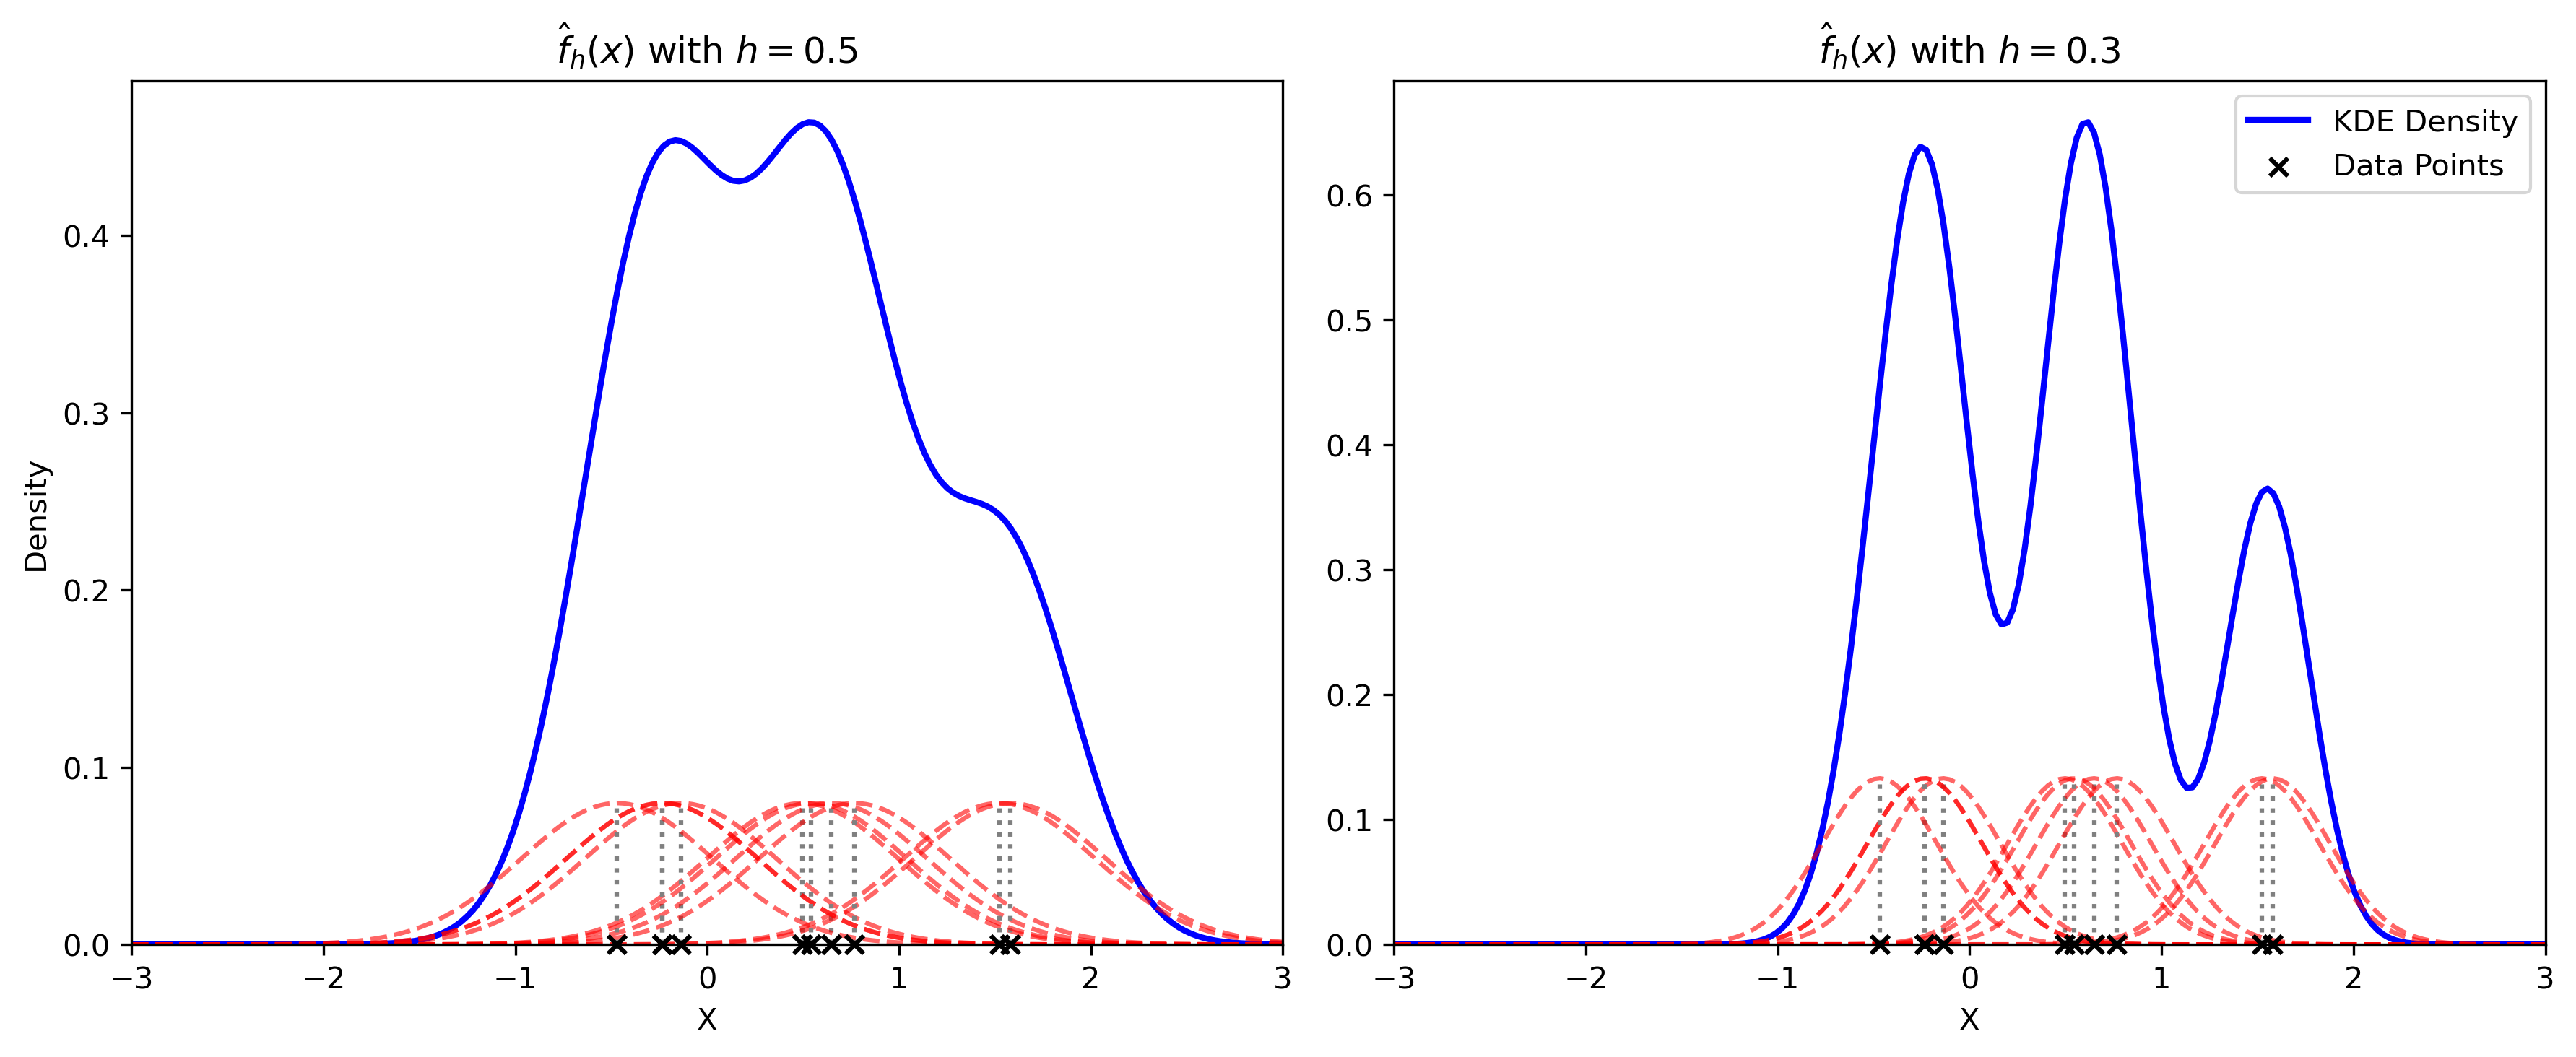
\includegraphics[width=\textwidth]{images/20_1.png}
  \end{minipage}
  \hfill
  \caption[Effect of bandwidth on KDE densities]{Higher bandwidth $h$ results in smoother density estimates. KDE from $n=5$ standard-normal draws, using Gaussian kernels with $h=0.5$ (left) and $h=0.3$ (right). Solid blue curves are the summed densities; dashed red curves are the individual kernels at each observation (black $\times$), and dotted vertical lines mark $\pm h$ around each point. A smaller $h$ preserves multimodal peaks, while a larger $h$ yields a smoother, lower-amplitude estimate.}
  \label{fig:combined1}
  \end{center}
  \end{figure}
The above makes it clear that a Gaussian kernel density estimator is nothing more than a sum of scaled Gaussians. This is a convenient opportunity to illustrate how the shape of $\hat{f_h}(x)$ varies as the bandwidth $h$ varies. Figure \ref{fig:combined1} demonstrates a set of 5 fictitious observations drawn from a standard normal distribution. Each observation is associated with a red Gaussian kernel, and the resulting blue density estimator is the sum of these kernels. Notably, a lower bandwidth results in a distinctly multimodal density, whereas a higher value of $h$ attenuates these peaks.
  


\subsection{Multivariate Case}

KDE also allows us to model multivariate empirical distributions, with the intuition remaining unchanged from the univariate case. Suppose we observe $n$ vectors $\mathbf{x}_i=(x_{i1}, x_{i2},...,x_{id})^\mathsf{T}$, where each vector is an observation drawn from an unknown $d$-variate distribution. The entire set of observations can be written as the matrix $\mathbf{X}=(\mathbf{x}_1,\mathbf{x}_2,...,\mathbf{x}_n)^{\mathsf{T}}\in\mathbb{R}^{n\times d}$. To estimate the probability density, we evaluate the kernel density estimator at a query point $\mathbf{x}=(x_{1}, x_{2},...,x_{d})\in\mathbb{R}^{d}$.

The multivariate KD estimator is thus defined in terms of some multivariate kernel function $K_\mathbf{H}(\mathbf{x})$ and $\mathbf{H}$ is the $d\times d$ symmetric positive definite bandwidth matrix:
$$\displaystyle\hat{f_h}(\mathbf{x})=\frac{1}{n}\sum_{i=1}^{n}K_\mathbf{H}(\mathbf{x}-\mathbf{x}_i)$$
Where $K_\mathbf{H}(\mathbf{x})$ is the scaled kernel function $K(\mathbf{x})$, so that:
$$\displaystyle K_\mathbf{H}(\mathbf{x})=\frac{1}{\sqrt{\det{(\mathbf{H})}}}K(\mathbf{{H}^\mathrm{-1/2}x})$$
When the Gaussian kernel is used, the KDE density is defined as:
$$\displaystyle\hat{f_h}(\mathbf{x})=\frac{1}{n}\sum_{i=1}^{n}\frac{1}{(2\pi)^{d/2}\sqrt{\det{(\mathbf{H})}}}\exp\left(-\frac{1}{2}\mathbf{(x-x_{\it{i}})^\mathsf{T}H^\mathrm{-1}(x-x_{\it{i}})}\right)$$

The bandwidth matrix $\mathbf{H}$ plays a role analogous to a covariance matrix, controlling the shape, orientation, and spread of the kernel functions. Its parametrization is arguably even more critical than the choice of the kernel. Three common configurations exist:

\begin{enumerate}
\item \textbf{Full bandwidth}: The most flexible form, which allows KDE to capture variations in dispersion and directional dependencies through the off-diagonal terms:
$$\mathbf{H}_{full}=\begin{pmatrix}h^2_1 & h_{12} & \cdots & h_{1d} \\ h_{12} & h^2_2 & \cdots & h_{2d} \\ \vdots & \vdots & \ddots & \vdots \\ h_{1d} & h_{2d} & \cdots & h^2_d\end{pmatrix}$$
This flexibility comes at the cost of increased complexity, requiring estimation of $d(d+1)/2$ parameters, which is feasible in lower dimensions but challenging as $d$ grows.

\item \textbf{Diagonal bandwidth}: A simplification that ignores covariance-like dependence, but still allows for heterogeneous dispersion across the $d$ random variables: 
$$\mathbf{H}_{diagonal}=\begin{pmatrix}h^2_1 & 0 & \cdots & 0 \\ 0 & h^2_2 & \cdots & 0 \\ \vdots & \vdots & \ddots & \vdots \\ 0 & 0 & \cdots & h^2_d\end{pmatrix}=\text{diag}(h^{2}_{1}, ..., h^{2}_{d})$$

\item \textbf{Isotropic bandwidth}: which imposes a uniform dispersion on every kernel with no explicit dependence:
$$\mathbf{H}_{isotropic}=\begin{pmatrix}h^2 & 0 & \cdots & 0 \\ 0 & h^2 & \cdots & 0 \\ \vdots & \vdots & \ddots & \vdots \\ 0 & 0 & \cdots & h^2\end{pmatrix}=h^2I$$
\end{enumerate}

There exist even more elaborate specifications of the bandwidth matrix $\mathbf{H}$, including bandwidth matrices specific to each observation $\mathbf{x}_i$, but we do not discuss these in the context of KDE. Crucially, a KDE estimator does not necessarily rely on the bandwidth matrix to model variable dependence. Instead, dependence arises naturally from the summation of kernels placed over observed data points. A visual example of this will be provided in Section \ref{sec:compare}.

Although the isotropic bandwidth may seem overly simplistic, it can be sufficient for constructing continuous density functions. A full bandwidth may be preferable when KDE is used for clustering, which is not our objective. For the subsequent portfolio analysis, we will use the diagonal bandwidth matrix.



\subsection{Bandwidth Selection via Cross-Validation}
\label{sec:crossval}
The quality of a KDE estimator is sensitive to the choice of the bandwidth matrix, and there are numerous methods for doing so algorithmically. We focus on cross-validation, which allows us to select each $h_i$ by maximizing the log-likelihood of estimators fit on subsets of the data over a fine grid of candidate values.

Concretely, for each random variable $i$ we partition its $n$ observed realizations $\{x_{1},...,x_{n}\}$ into $k$ disjoint folds, and denote by $I_{c}$ the set of indices in fold $c$. For each candidate bandwidth $h$ we then compute the cross-validated score
$$
\mathrm{CV}(h)=
\frac{1}{k}
\sum_{c=1}^{k}
\sum_{j \,\in\, I_c}
\log\left(\hat{f}_{-c,h}(x_j)\right),
$$
Where $\hat{f}_{-c,h}$ denotes the KDE fitted on all data except those in fold $c$, using bandwidth $h$. We then set
$$
\hat{h}_i = 
\arg\max_h\;\mathrm{CV}(h).
$$

In preliminary experiments across our five index universes, each $\hat{h}_i$ aligned almost exactly with the sample standard deviation $\sigma_i$ of the corresponding realization series. To reduce computational time, we therefore fix $\mathbf{H}=\mathrm{diag}\bigl(\sigma_{1}^{2}, \dots, \sigma_{d}^{2}\bigr)$ for all subsequent empirical tests.

\section{Moments}
\label{sec:momentsec}
We will need the mean and variance of a portfolio projection $\mathbf{\alpha^{\mathsf{T}}x}$ under a KDE density (useful in \ref{sec:tangency}). To derive these, working with the moment-generating function (MGF) is convenient. We fix a weight vector $\alpha\in\mathbb R^d$ and let
$$
Y=\alpha^{\mathsf{T}} X,\quad
\hat f(x)=\frac1n\sum_{i=1}^n\mathcal N(x\mid x_i,H).
$$
The moment-generating function of $Y$ is simply the sum of the MGFs of the Gaussian density
$$
M(u)=\mathbb E[e^{uY}]
=\int \exp\bigl(u\,\alpha^{\mathsf{T}} X\bigr)\,\hat f(x)\,dx
=\frac1n\sum_{i=1}^n\exp\!\Bigl(u\,\alpha^{\mathsf{T}} x_i+\tfrac12\,u^2\,\alpha^{\mathsf{T}} H\,\alpha\Bigr).
$$
Taking the first derivative, and evaluating at $u=0$:
$$
M'(u)
=\frac1n\sum_{i=1}^n
\exp\!\Bigl(u\,\alpha^{\mathsf{T}} x_i+\tfrac12\,u^2\,\alpha^{\mathsf{T}} H\,\alpha\Bigr)
\Bigl(\alpha^{\mathsf{T}} x_i+u\,\alpha^{\mathsf{T}} H\,\alpha\Bigr).
$$
$$
M'(0)
=\frac1n\sum_{i=1}^n(\alpha^{\mathsf{T}} x_i)
=\alpha^{\mathsf{T}}\bar x.
$$
Thus:
$$\mathbb{E}[\alpha^{\mathsf{T}} X] = \alpha^{\mathsf{T}} \bar x$$

Now differentiate $M'(u)$ and evaluate at $u=0$ once more to get the second central moment:
$$
M''(u)
=\frac1n\sum_{i=1}^n
\exp\!\Bigl(u\,\alpha^{\mathsf{T}} x_i+\tfrac12\,u^2\,\alpha^{\mathsf{T}} H\,\alpha\Bigr)
\Bigl((\alpha^{\mathsf{T}} x_i+u\,\alpha^{\mathsf{T}} H\,\alpha)^2
+\alpha^{\mathsf{T}} H\,\alpha\Bigr).
$$
$$
M''(0)
=\frac1n\sum_{i=1}^n\Bigl((\alpha^{\mathsf{T}} x_i)^2+\alpha^{\mathsf{T}} H\,\alpha\Bigr)
=\alpha^{\mathsf{T}} H\,\alpha+\frac1n\sum_{i=1}^n(\alpha^{\mathsf{T}} x_i)^2.
$$
Using $\mathrm{Var}(Y)=M''(0)-[M'(0)]^2$,
$$
\mathrm{Var}(\alpha^{\mathsf{T}} X)
=\alpha^{\mathsf{T}} H\,\alpha
+\frac1n\sum_{i=1}^n(\alpha^{\mathsf{T}} x_i)^2
-\bigl(\alpha^{\mathsf{T}}\bar x\bigr)^2.
$$
Noting that the sample covariance $S=\frac1n\sum_i(x_i-\bar x)(x_i-\bar x)^{\mathsf{T}}$ satisfies the equality
$\frac1n\sum_i(\alpha^{\mathsf{T}} x_i)^2-(\alpha^{\mathsf{T}}\bar x)^2=\alpha^{\mathsf{T}} S\,\alpha$, we obtain:

\begin{equation}\label{eq:kdevar}
  \mathrm{Var}(\alpha^{\mathsf{T}} X)=\alpha^{\mathsf{T}}\bigl(H+S\bigr)\alpha.
\end{equation}


\section{Gaussian Mixture Models}
\subsection{Multivariate Case}
Mixture models are similar to KDE in that they approximate the distribution of a random variable as a sum of scaled kernel functions. As in KDE, various kernel functions can be used, but we focus exclusively on the Gaussian Mixture Model (GMM).

The key difference is that KDE places a kernel at each of the $n$ observations, whereas GMM models the data as arising from $K$ Gaussian components, where $K$ is typically much smaller than $n$. Each component in GMM has a distinct mean vector $\mathbf{\mu_{\it{i}}}$ and covariance matrix $\mathbf{\Sigma_{\it{i}}}$, whereas in KDE, all kernels share a common bandwidth matrix $\mathbf{H}$ and differ only in their centering vectors $\mathbf{x_{\it{i}}}$. Additionally, each Gaussian component $i$ is assigned a weight $\phi_i$, representing its proportion in the mixture, with $\sum_{i=1}^{K}\phi_{i}=1$.

Defining the parameter set as $\mathbf{\theta}=\{ \mathbf{\phi_{\it{i}},\mu_{\it{i}},\mathbf{\Sigma_{\it{i}}}}\}^K_{i=1}$, the multivariate density function generated by GMM is:

$$\displaystyle\hat{f}_{GMM}(\mathbf{x|\theta})=\sum_{i=1}^{K}\phi_{i} \mathcal{N}(\mathbf{x|\mu_{\it{i}},\Sigma_{\it{i}}})$$

Where $\mathcal{N}(\mathbf{x|\mu_{\it{i}},\Sigma_{\it{i}}})$ is the multivariate normal density. Thus, the full GMM function is:

$$\displaystyle\hat{f}_{GMM}(\mathbf{x|\theta})=\sum_{i=1}^{K}\phi_i\frac{1}{(2\pi)^{d/2}\sqrt{\det{(\mathbf{\Sigma_{\it{i}}})}}}\exp\left(-\frac{1}{2}\mathbf{(x-\mu_{\it{i}})^\mathsf{T}\Sigma_{\it{i}}^\mathrm{-1}(x-\mu_{\it{i}})}\right)$$

Hence, GMM and KDE are equivalent if $K=n$, $\phi_{i}=1/n$, $\mathbf{\Sigma}_i=\mathbf{H}$ and $\mathbf{\mu_{\it{i}}=x_{\it{i}}}$ for all $i$.

\subsection{Parameter Estimation via Expectation–Maximization}

For a fixed mixture order $K$, the GMM parameters $\theta = \{\phi_i,\mu_i,\Sigma_i\}_{i=1}^K$ are estimated by maximum likelihood using the EM algorithm, as shown by \cite{rednerMixtureDensitiesMaximum1984}. Starting from an initial guess, EM iterates between two steps until convergence:

\begin{enumerate}
\item \textbf{E-step}: Using the current mixture weights $\phi_i$, means $\mu_i$, and covariances $\Sigma_i$, compute for each observation $x^{(j)}$ how likely it is to come from each component. Concretely, you calculate a score for component $i$ by combining its weight and its Gaussian density at $x^{(j)}$, then normalize these scores across all $K$ components to obtain the so-called responsibility $\tau_i(x^{(j)})$.

For each data point $x^{(j)}$, compute the responsibilities with

$$
\tau_i\bigl(x^{(j)}\bigr)
= \frac{\psi_i(x^{(j)})}
{\sum_{k=1}^K \!\psi_k(x^{(j)})},
$$

where $\psi_i(x^{(j)})$ is the unnormalized score for component $i$, observation $j$:
$$
\psi_i\bigl(x^{(j)}\bigr)=
\phi_i\,\mathcal{N}\bigl(x^{(j)}\mid\mu_i,\Sigma_i\bigr).
$$ 
\item \textbf{M-step}: Treating the responsibilities $\tau_i(x^{(j)})$ as weights, update each of the $K$ component's parameters: 
  \begin{itemize}
    \item Mixture weight: $\phi_i$ becomes the average responsibility over all observations. 
    \item Mean: $\mu_i$ becomes the weighted average of the data, using $\tau_i(x^{(j)})$.
    \item Covariance: $\Sigma_i$ becomes the weighted sample covariance around the new mean, again using the responsibilities.
  \end{itemize}
$$
\phi_i \;\leftarrow\;
\frac{1}{n}\sum_{j=1}^n 
\tau_i\bigl(x^{(j)}\bigr),
\quad
\mu_i \;\leftarrow\;
\frac{\sum_{j=1}^n 
\tau_i\bigl(x^{(j)}\bigr)\,
x^{(j)}}{\sum_{j=1}^n 
\tau_i\bigl(x^{(j)}\bigr)},
\quad
$$
$$
\Sigma_i \;\leftarrow\;
\frac{\sum_{j=1}^n 
\tau_i\bigl(x^{(j)}\bigr)\,
(x^{(j)}-\mu_i)(x^{(j)}-\mu_i)^{\!\mathsf{T}}}
{\sum_{j=1}^n 
\tau_i\bigl(x^{(j)}\bigr)}
$$
\end{enumerate}

Each iteration increases the observed log-likelihood. The algorithm terminates when the change in log-likelihood (or in $\theta$) falls below a pre-specified tolerance.

Thankfully, practitioners can rely on off-the-shelf software packages to perform this procedure. We relied on SciPy's highly optimized \textit{GaussianMixture} implementation, although fitting still proved slow for the scope of our analysis, especially for large asset universes.

\subsection{Model Selection}
\label{sec:gmmselect}
Choosing the number of components K requires balancing goodness-of-fit against model complexity. We evaluate candidate mixtures via the Akaike Information Criterion
$$\mathrm{AIC} = -2\,\ell(\hat\theta) + 2\,p,$$
and the Bayesian Information Criterion
$$\mathrm{BIC} = -2\,\ell(\hat\theta) + p\,\log(n),$$
where $\ell(\hat\theta)$ is the maximized log-likelihood, $p$ the number of free parameters, and $n$ the sample size. In our preliminary tests in subsets of the data, BIC almost always selected $K$=1 (the single Gaussian case), while AIC sometimes preferred larger $K$. To maintain focus on actual mixture models, and to avoid the need to recompute the EM algorithm for each feasible $K$, we fix $K$=8 (or $K$=$\min(8,n)$) for all further analysis.

\section{Comparative Illustration: KDE vs. GMM}
\label{sec:compare}
Now that we have defined both approaches, it is worth discussing their differences and applicability to modeling returns of financial assets. First, we demonstrate the computational tradeoffs. Below is a diagram of 300 simulated data points drawn from an equally weighted combination of normal distributions with different means and covariance matrices:
$$
X=(x_1,x_2)^\mathsf{T} \sim \tfrac12\,\mathcal N(\mu_1,\Sigma_1)\;+\;\tfrac12\,\mathcal N(\mu_2,\Sigma_2),
$$
$$\mu_1 = \bigl(\!\begin{smallmatrix}-3\\-3\end{smallmatrix}\!\bigr),\;\Sigma_1 = \bigl[\!\begin{smallmatrix}1 & -0.9\\-0.9 & 1\end{smallmatrix}\!\bigr],\;\mu_2 = \bigl(\!\begin{smallmatrix}3\\3\end{smallmatrix}\!\bigr),\;\Sigma_2 = \bigl[\!\begin{smallmatrix}1 & 0.9\\0.9 & 1\end{smallmatrix}\!\bigr]$$


\begin{figure}[H]
  \centering
  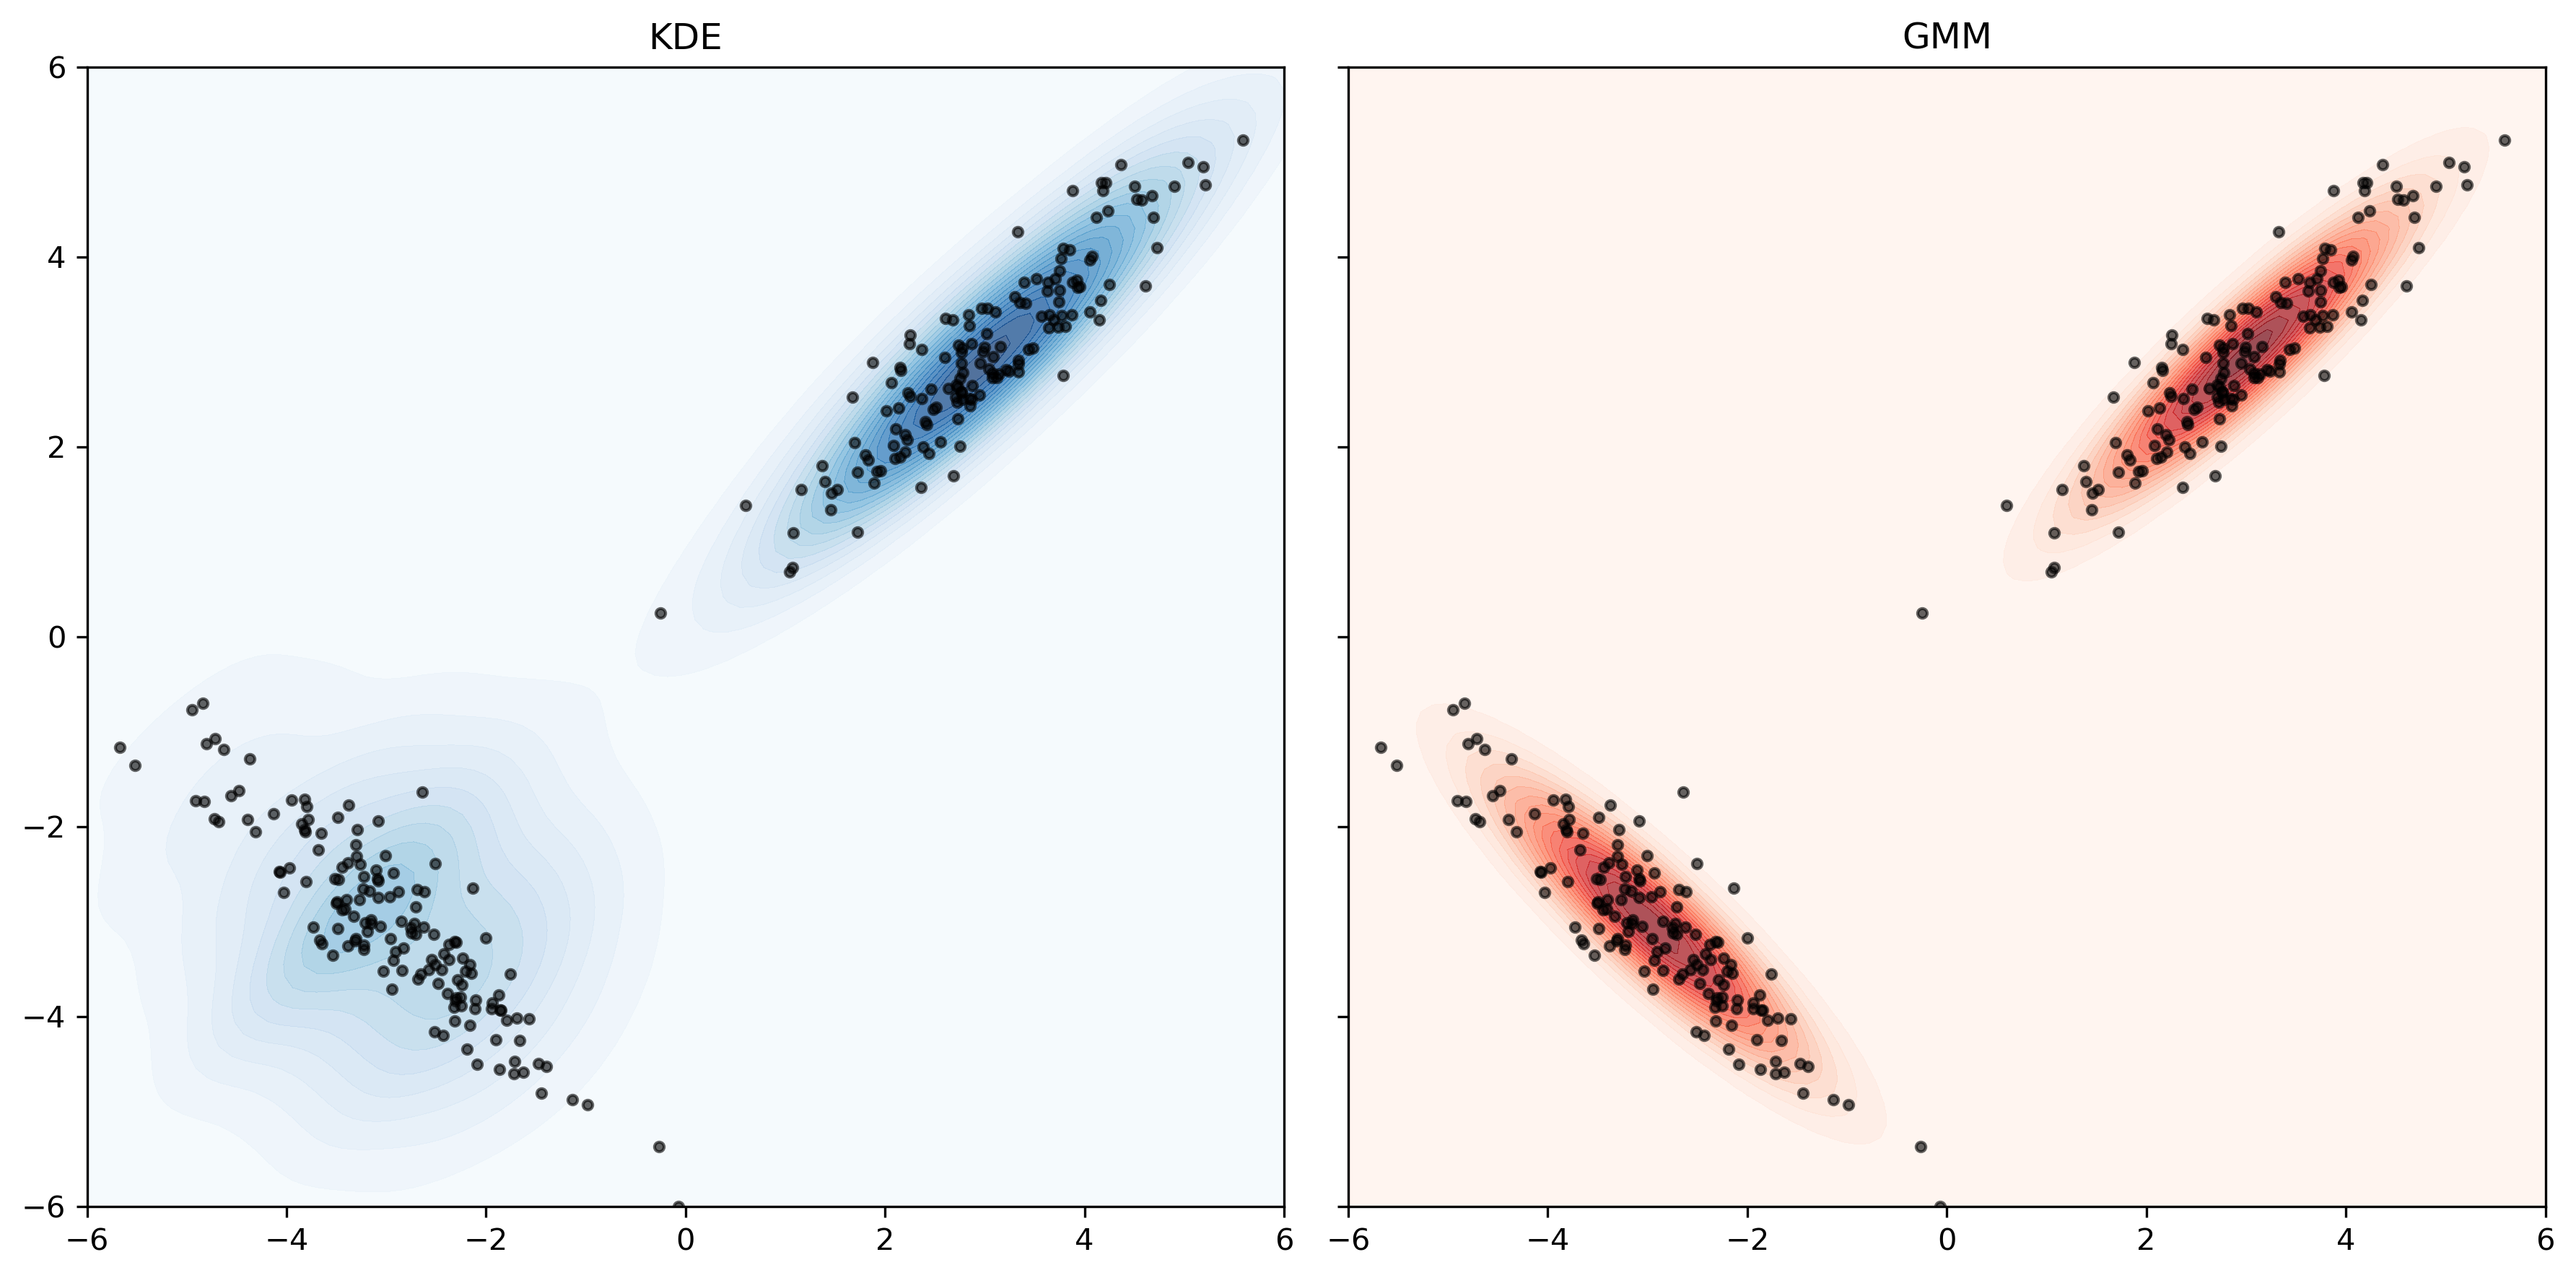
\includegraphics[width=\textwidth]{images/20_2.png}
  \caption[Best case scenario - GMM]{A two-component GMM more accurately recovers two correlated clusters than KDE. KDE (left, blue) and GMM densities (right, red; 2 components) for 300 samples drawn from two bivariate normals (150 points each) with strong negative and positive correlations. Colored filled contours show the estimated density; black dots are the data.}
  \label{fig:10_3}
\end{figure}

Both KDE and GMM describe the two-cluster structure (\ref{fig:10_3}) well, but GMM does so with only $K$=2 components, against KDE's $n$=300 kernels. When data exhibit clear Gaussian clusters, GMM is far more parsimonious; however, such distinct multimodality rarely occurs in financial returns. There is a tradeoff between GMM's parametric efficiency and KDE's nonparametric flexibility. GMM components remain strictly elliptical by construction, whereas KDE contours adapt to local data shape.

The parsimony of GMM can become a limitation when the data structure is highly nonlinear. In the following example, we present a noisy circular distribution that illustrates this, again drawing 300 observations. Each point's radial distance from the origin follows a normal distribution centered at $3$ with a standard deviation of $0.3$, while the angular positions are uniformly distributed over $[0, 2\pi]$:
$$\displaystyle (\begin{smallmatrix} x_1 \\ x_2 \end{smallmatrix}) = \left(3 + \epsilon\right) (\begin{smallmatrix} \cos\theta \\ \sin\theta \end{smallmatrix}), \quad \theta \sim \text{Uniform}(0, 2\pi), \quad \epsilon \sim \mathcal{N}(0, 0.3^2)$$

\begin{figure}[H]
  \centering
  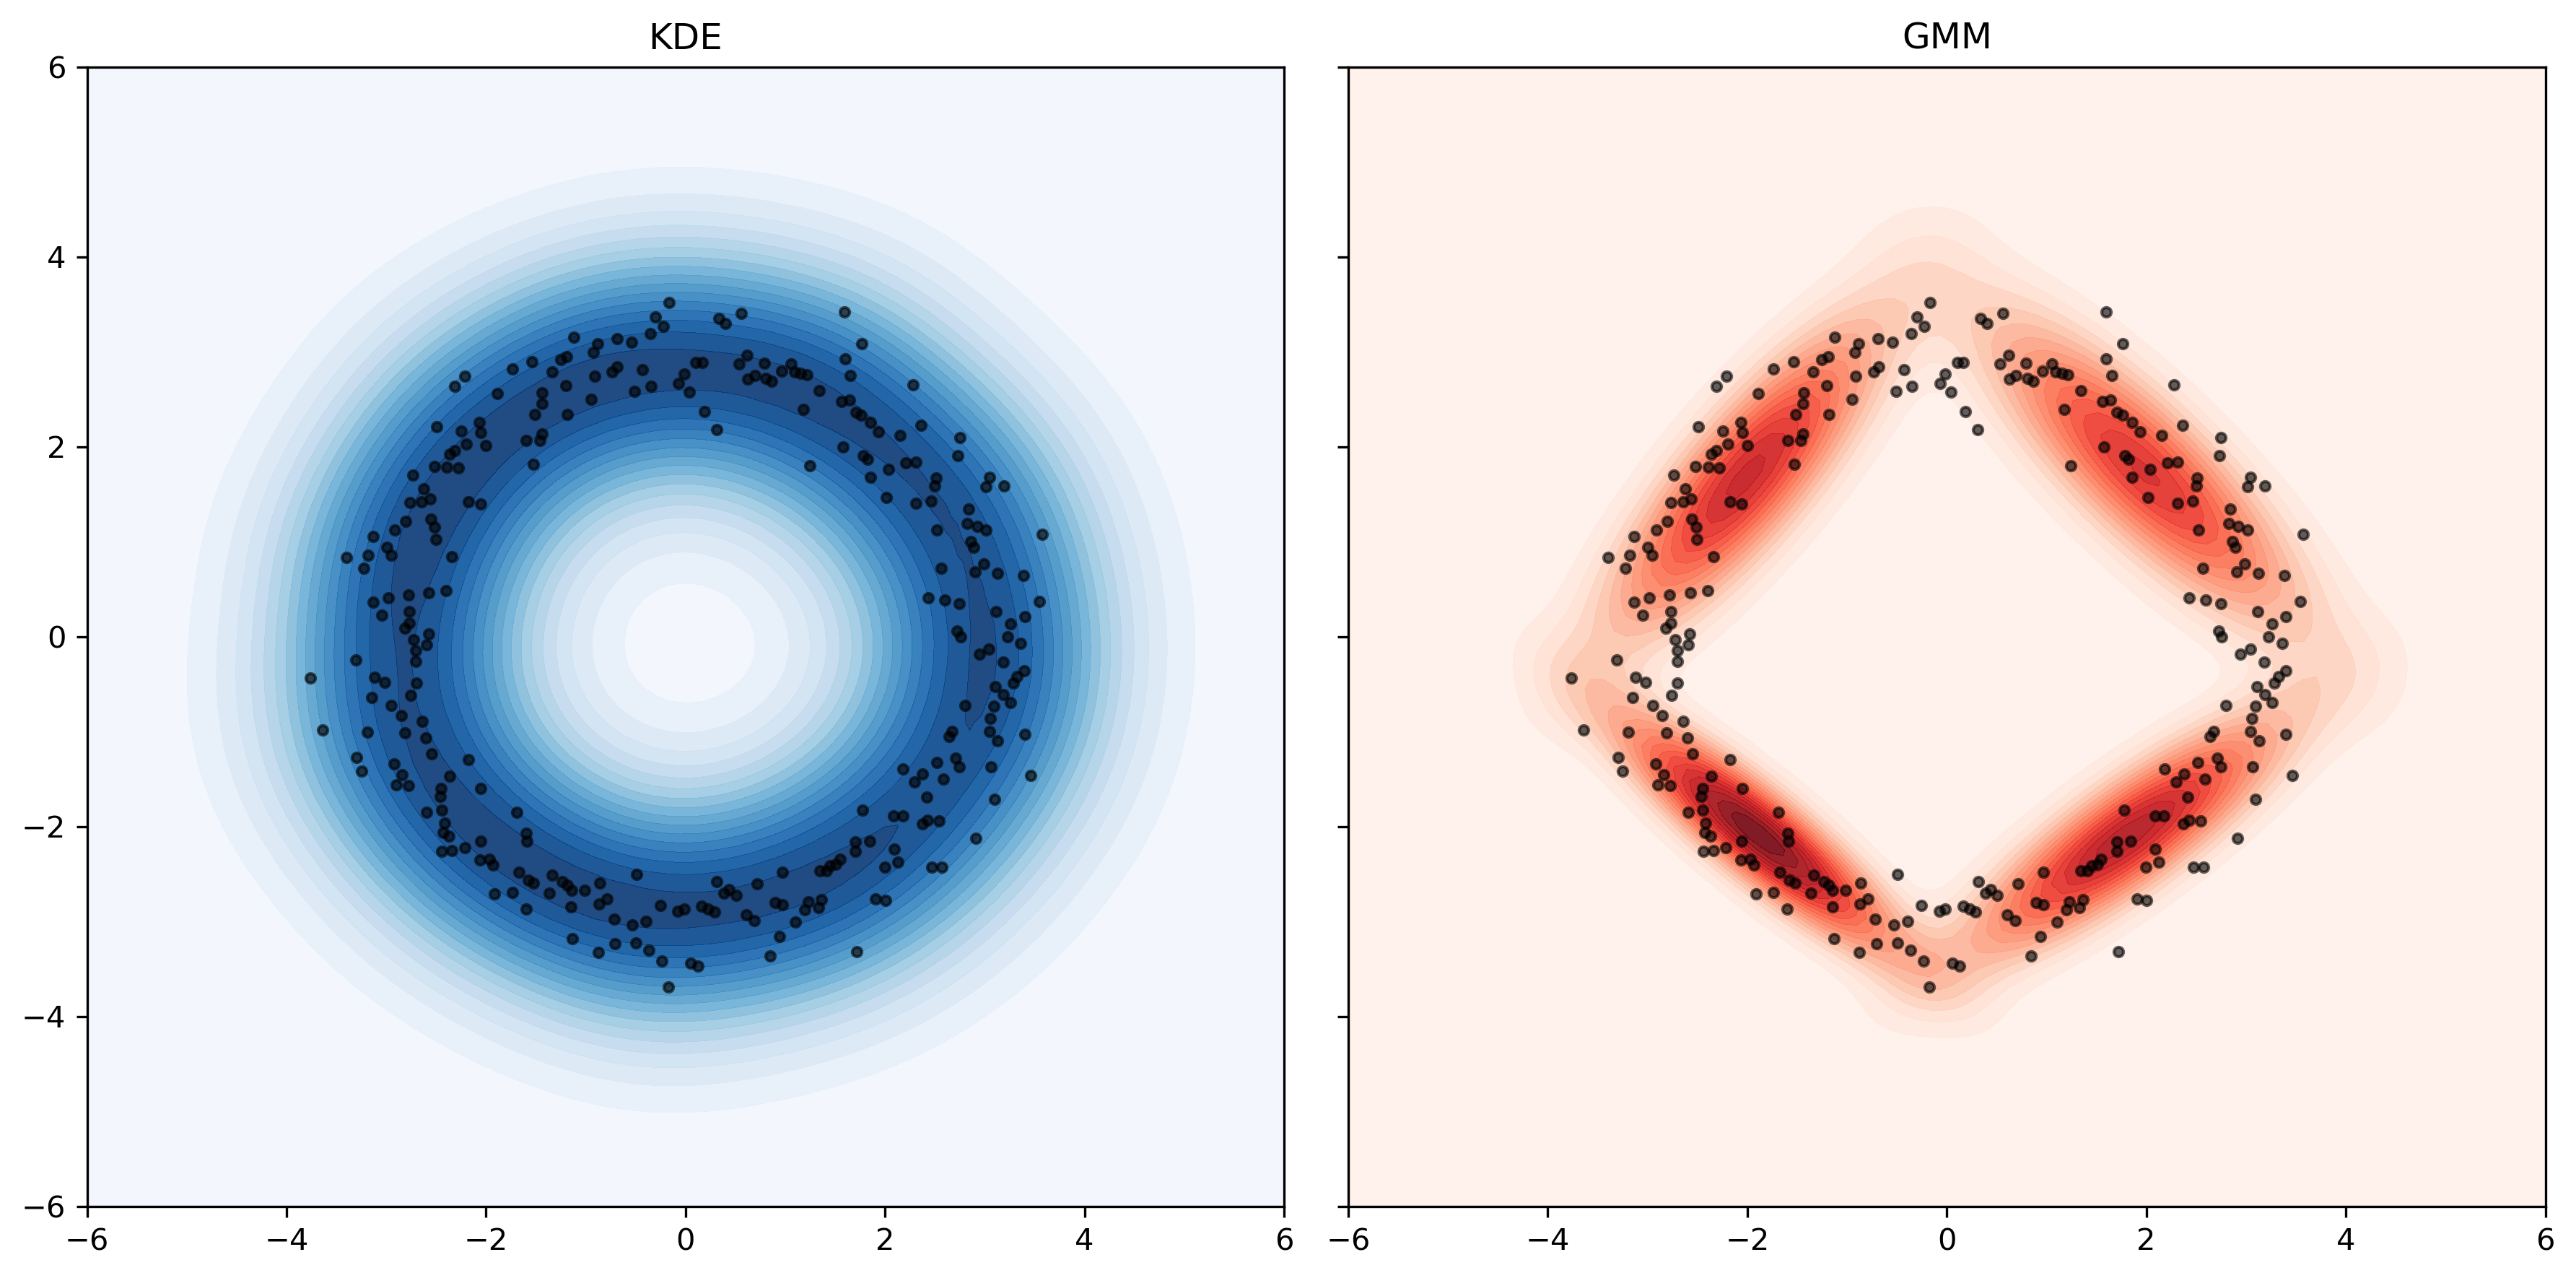
\includegraphics[width=\textwidth]{images/20_3.png}
  \caption[Best case scenario - KDE]{KDE captures a continuous ring-shaped density that GMM decomposes into discrete blobs. KDE (left, blue) and GMM (right, red; 4 components) for 300 points sampled around a noisy circle of radius $\approxeq$3. Colored filled contours show the estimated density; black dots are the data. }
  \label{fig:10_4}
\end{figure}

In this example, we used $K=4$ GMM components, which is evidently insufficient to describe the circular distribution. Increasing $K$ would reduce this bias, but at the cost of greater computational complexity. Therefore, when modeling data that exhibits nonlinear dependence structures, KDE's flexibility may outweigh GMM's theoretical efficiency.

In the context of our portfolio optimization framework (Chapter~\ref{chap:portfolio}), the use of a KDE density is usually significantly faster than GMM, especially as the window size grows large. The pitfall of GMM is the model estimation step, which quickly overshadows the higher cost of KDE at the optimization step. Inquisitive readers may refer to Appendix \ref{app:compute} for more on computational aspects.

\subsection{Log-Sum-Exponent and Softmax}
In Chapter~\ref{chap:portfolio}, we will encounter the log-sum-exponent (LSE) operator as the key building block of our portfolio objective. To prepare, we introduce it here and summarize its main properties. The complete derivation of its gradient and Hessian is given in Appendix~\ref{app:lse}.

Let $f(\mathbf{w})=(f_1(\mathbf{w}), f_2(\mathbf{w}),...,f_k(\mathbf{w}))^{\mathsf{T}}$ be a vector valued, twice-differentiable function. The log-sum-exponent operator of $f$ is defined as:
$$LSE_i(f_i(\mathbf{w}))=\log{\sum_{i=1}^{k}\exp(f_i(\mathbf{w}))}$$

Associated with LSE is the softmax function, which produces a probability distribution over the indices $i=1,...,k$:
$$\mathrm{softmax}_i(f)=p_i=\frac{{\exp( f_i(\mathbf{w}))}}{\sum_{i=1}^{k}\exp (f_i(\mathbf{w}))}$$
Softmax acts as a smooth approximation to the max operator, in that it concentrates weight on the largest components (\cite{boydConvexOptimization2004}).

$\textbf{Gradient of LSE}$: 
\newline
Define
$$S=\sum_{i=1}^k \exp{f_i(\mathbf w)}.$$
Then
$$\nabla_\mathbf w\,\mathrm{LSE}(f) = \nabla_\mathbf w\log S = \frac{1}{S}\,\nabla_\mathbf w S = \sum_{i=1}^k p_i\,\nabla f_i(\mathbf w).$$
In other words, the gradient of LSE is the softmax-weighted average of the individual gradients $\nabla f_i$.

$\textbf{Hessian of LSE}$: 
\newline
The Hessian matrix $\nabla^2 \mathrm{LSE}(f)$ can be expressed in terms of the component Hessians and gradients:
$$\nabla^2 \mathrm{LSE}(f) = \sum_{i=1}^k p_i \bigl[\nabla^2 f_i + (\nabla f_i)(\nabla f_i)^{\mathsf{T}}\bigr] \cdot \Bigl(\sum_{i=1}^k p_i\,\nabla f_i\Bigr)\Bigl(\sum_{j=1}^k p_j\,\nabla f_j\Bigr)^{\mathsf{T}}$$
One can show (Appendix~\ref{app:lse}) that so long as $f(\mathbf{w})$ is convex, this matrix is positive semidefinite and therefore convex.